\section{Наибольшая общая Абелева подстрока}
% Описываешь задачу

\subsection{Общий алгоритм}

В качестве решения задачи нас будут интересовать только детерминированные алгоритмы решения задачи. Известно несколько недетерминированных решений, на практике работающих достаточно быстро, но они не являются темой исследования данной работы.

%Мы будем описывать алгоритмы по шагам, начиная от самого медленного решения.
Будем подходить к лучшему решению по шагам от самого простого, на каждом шаге оптимизируя какую-то часть алгоритма, для лучшего понимания.

\subsubsection{$\langle \mathcal{O}(n^2 \log \sigma), \mathcal{O}(n \log \sigma) \rangle$ w.h.p}

Будем перебирать длину $l$ и проверять, есть ли общая Абелева подстрока длины $l$.
Сформулируем план. Мы будем строить $\mathcal{P}(t)$ для всех подстрок $t$ длины $l$ от $1$ до $n$ строк $a$ и $b$, потом проверять, есть ли две строки с одинаковым $\mathcal{P}(t)$.

Будем строить векторы $\mathcal{P}(t)$ для всех подстрок длины $l$ строк $a$ и $b$ по очереди, переходя от одной подстроки к следующей. Для этого нужно уметь удалять первый символ текущей подстроки и дописывать в конец новый символ. Расширим алфавит на один символ, добавив разделитель $\$$, нигде ранее не встречавшийся, и будем идти скользящим окном длины $l$ по строке $a\$b$.

Хранить векторы $\mathcal{P}(t)$ будем в персистентном массиве длины $\sigma$, реализованном на персистентном дереве отрезков. Для того, чтобы перейти к следующей подстроке, нужно уменьшить число в ячейке, соответствующей удаляемому символу, на 1, и увеличить значение в ячейке, соответствующей добавляемому символу, на 1.

Для того, чтобы научиться сравнивать на равенство два корня дерева, соответствующие двум векторам $\mathcal{P}(t)$, будем при построении считать некоторое число $h(v)$~--- класс эквивалентности всех вершин дерева. Этот класс эквивалентности будет соответствовать набору значений на подотрезке символов, соответствующему этой вершине дерева отрезков~--- две вершины в одном классе эквивалентности, если они соответствуют одному и тому же подотрезку символов, и число вхождений каждого символа у них одинаково.

Будем поддерживать хешмап, в котором для пары чисел $\langle h_1, h_2 \rangle$ хранится класс эквивалетности этой пары, если она уже встречалась. Чтобы посчитать хеш для листа, получим класс эквивалентности у пары $\langle -pos, val \rangle$, где $pos$~--- номер символа, соответствующего этому листу, а $val$~--- значение, записанное в этой вершине. Такая пара, с отрицательным $-pos$, выбирается для того, чтобы избежать коллизии со внутренними вершинами, характеристиками которых являются пары неотрицательных чисел~--- пара уже посчитанных классов эквивалентности сыновей $\langle h(v_l), h(v_r) \rangle$, где $v_l$~--- левый сын вершины, а $v_r$~--- правый сын вершины. Когда нам нужно узнать хеш пары $\langle h_1, h_2 \rangle$, смотрим в хешмап: если там есть элемент с таким ключом, то соответствующий класс эквивалентности уже посчитан, иначе кладем туда новый элемент с таким ключом и значением, равным размеру хешмапа. Значения всех хешей таким образом будут принимать значения от $0$ до $MapSize - 1$, где $MapSize$~--- текущий размер хешмапа, не превышающий $\mathcal{O}(n \log \sigma)$.

Таким образом, после подсчета класса эквивалентности каждой вершины, для всех подстрок длины $l$ первой и второй строки можно выписать их классы эквивалентности, а именно, значения в корнях персистентного дерева. Теперь нужно проверить, есть ли в двух массивах одинаковое число. Поскольку все значения имеют порядок $\mathcal{O}(n \log \sigma)$, это можно сделать, используя сортировку подсчетом.

Время работы~--- $n$ итераций по $l$, и $\mathcal{O}(n \log \sigma)$ операций для каждой длины: вычисление класса эквивалентности каждой вершины дерева отрезков работает за $\mathcal{O}(1)$ w.h.p. используя обращение хешмапу. Расходуемая память $\mathcal{O}(n \log \sigma)$ на хранение дерева отрезков и хешмапа.


\subsubsection{$\langle \mathcal{O}(n^2 \log \sigma), \mathcal{O}(n^2) \rangle$ deterministic}

Посмотрим внимательнее на персистентное дерево отрезков из предыдущего решения. Это ациклический ориентированный граф, в котором каждая вершина имеет свой уровень (глубину) от $1$ до $\log \sigma$, при чем на каждой глубине находится $\mathcal{O}(n)$ вершин.

Будем считать классы эквивалентности всех вершин, поднимаясь по уровням от листьев к корням, используя один хешмап размера $\mathcal{O}(n^2)$, который умеем очищать за $\mathcal{O}(1)$. В этом подразделе под хешмапом я подразумеваю просто массив на $\mathcal{O}(n^2)$ элементов с пометкой последнего изменения для возможности обнуления за $\mathcal{O}(1)$.

В этом решении класс эквивалентности будет иметь не сквозную нумерацию среди всех вершин дерева, как в предыдущем решении, а иметь отдельную нумерацию для каждого уровня вершин дерева.

Начнем с самого низкого уровня. Посчитаем классы эквивалентности листьев. Класс эквивалентности листа, как и в прошлом пункте, $h(\langle -pos, val \rangle)$, где и $pos$, и $val$ принимают значения порядка $\mathcal{O}(n)$. Поэтому можно пройти по всем листьям в дереве, и посчитать классы, обращаясь к хешмапу напрямую и спрашивая, был ли уже такой же лист, и какой у него класс эквивалентности. Для того, чтобы обойти все листы за их число, при изменении значения в листе можно в лист складывать ссылку на новый лист, который появляется в следующей версии дерева отрезков.

Опишем переход от одного уровня к следующему. Допустим, уже посчитан класс эквивалентности всех вершин более глубокого уровня. Обратим внимание, что поскольку на каждой глубине $\mathcal{O}(n)$ вершин, классы этих вершин так же будут принимать значения $\mathcal{O}(n)$. Поэтому мы можем очистить хешмап и точно так же, как и для листьев, считать значение класса, к которому относится вершина, проверяя, была ли уже такая пара $\langle h(v_l), h(v_r) \rangle$.

Таким образом, мы построили дерево и посчитали хеши всех вершин за $\langle \mathcal{O}(n^2 \log \sigma), \mathcal{O}(n^2) \rangle$ полностью детерменированно.


\subsubsection{$\langle \mathcal{O}(n^2 \log \sigma), \mathcal{O}(n) \rangle$ deterministic}

Начнем с того, что на хранение дерева отрезков у нас сейчас уходит $n \log \sigma$ памяти, и это много. Чтобы уменьшить потребление памяти, можно использовать технику \textbf{limited node copying}. Кратко опишем эту технику, поскольку это будет необходимо для дальнейшего понимания алгоритма. 

Вместо того, чтобы после пересоздания очередного листа пересоздавать весь путь до корня, будем хранить в каждой вершине дополнительный указатель, изначально нулевой. При изменении значения в листе будем подниматься по предкам, пока у предка дополнительный указатель уже занят, и создавать в этом случае новую вершину. Когда мы стоим в вершине и знаем, что один из ее сыновей был изменен, а дополнительный указатель еще не занят, просто установим этот дополнительный указатель на новую версию этого сына и подпишем текущим глобальным временем. После такого изменения все еще несложно обратиться к какой-то версии дерева отрезков: нужно просто при переходе к сыновьям при выборе, куда спускаться, посмотреть, не нужно ли идти по дополнительному указателю.

Можно доказать, что таким образом построенное дерево занимает $\mathcal{O}(n)$ памяти, используя амортизационный анализ, но не будем об этом. 

Подсчет классов эквивалентности для листьев и внутренних вершин в этом решении отличается.

Начнем с самого низкого уровня, а именно построим классы эквивалентности для листьев. Будем считать классы для листьев группами, для каждой позиции все листья, соответствующие этой позиции в массиве, вместе. Будем поддерживать счетчик $ch$~--- первый еще не использованный номер класса эквивалентности. Фиксировав позицию, которую мы сейчас обрабатываем, обойдем все листья с этой позицией (для этого можно хранить в каждом листе ссылку на предыдущий лист этой позиции), и листу со значением $val$ присвоим класс $ch+val$. После этого увеличим $ch$ на $maxValue_{pos}+1$, где $maxValue_{pos}$~--- наибольшее значение, которое было в ячейке $pos$ в одной из версий дерева отрезков. Мы знаем $maxValue_{pos}$ для каждой позиции, и можно заметить, что число классов эквивалентности на этом уровне $\mathcal{O}(n)$, поскольку $\sum \limits_{pos=1}^{\sigma} maxValue_{pos} = \mathcal{O}(n)$.

Опишем переход от одного уровня к следующему. Допустим, мы посчитали классы для всех (даже больше, чем для всех вершин, об этом далее) вершин на предыдущем уровне. После завершения очередного уровня, будем передавать на уровень выше не только посчитанные классы эквивалентности всех вершин, но и все не созданные явно из-за \textbf{limited node copying} копии вершин. Этот момент стоит описать более подробно, потому что сделать это не совсем тривиально. 

Рассмотрим момент, когда мы развернули очередной уровень дерева, создав все несозданные явно вершины этого слоя.

\begin{lemma}
Каждая вершина в сжатом персистентном дереве соответствует набору вершин, отвечающих за такой же отрезок символов в несжатом дереве, созданных в некоторый промежуток времени $[t_1; t_2)$, причем для всех вершин несжатого дерева, отвечающих за этот отрезок, эти промежутки времен не пересекаются.
\end{lemma}

\begin{proof}
Рассмотрим <<срез>> персистентного дерева в некоторый момент времени. Срез дерева в момент времени~--- дерево без дополнительных ссылок, в котором один из сыновей заменен на вершину по дополнительной ссылке, если на этой ссылке написано время не большее, чем момент среза. Поскольку именно такой срез дерева поддерживался при построении, легко понять, что вершина <<живет>> в сжатом дереве с момента создания до момента замены на свою новую версию, и отвечает за отрезок времен, соответствующих всем изменениям в ее поддереве, произошедших за ее время жизни.
\end{proof} 

Теперь опишем, как передавать отрезки версий вершин предкам в алгоритме.
За время жизни вершины у нее несколько раз меняются предки в текущем срезе персистентного дерева (предок меняется, если произошло изменение в другом сыне предка, и у предка не осталось дополнительного указателя). В алгоритме, когда мы развернули каждую вершину, создав все ее явные копии, нужно для каждого ее предка отправить такой подотрезок этих копий, который соответствует моментам времени, когда данный предок являлся предком текущей неявной вершины. Поскольку все эти моменты времени не пересекаются, можно явно передать всем предкам информацию о том, что в такие времена у вершины сыном была такая-то вершина, суммарно мы передадим все на следующий уровень за $\mathcal{O}(n)$ памяти и времени. Потом нужно будет в вершине-предке отсортировать все пришедшие данные из потомков, но поскольку это объединение не больше трех отсортированных массивов (информация приходила только из непосредственного сына, а их всего три с учетом дополнительного указателя), это можно так же сделать за линейное время.

%, разворачивая один уровень сжатого персистентного дерева отрезков. 
Поскольку без оптимизаций на каждом уровне линейное количество вершин, после создания всех неявных вершин их останется линейное число. При переходе на послеследующий уровень все эти вершины можно удалить, чтобы сохранить линейную память.
Чтобы получить для вершины список всех интересных времен, и понять, сколько ее копий нужно сделать, нужно объединить список всех времен у сыновей и у дополнительного указателя, если он есть. 

Следующее, что нужно сделать~--- сгруппировать все вершины с одинаковым $h(v_l)$ в одну группу, и обработать их вместе, чтобы назначить им соответствующие классы эквивалентности. Пусть у очередной вершины (для каждого варианта глобального времени, которое в ней интересно) классы сыновей $h(v_l)$ и $h(v_r)$. Запишем в вектор с номером $h(v_l)$ напоминание: нужно посчитать $h(\langle h_1, h_2 \rangle)$ и записать его в текущую вершину $v$. После того, как мы сделали это для всех вершин текущего уровня, нужно перебрать $h(v_l)$, создать хешмап размера $\mathcal{O}(n)$ (на самом деле, можно использовать один и тот же, просто очищая его за $\mathcal{O}(1)$), и перебрать соответствующее ему $h(v_r)$, назначая вершинам текущего уровня соответствующие классы. Как обычно, если $h(v_r)$ есть в хешмапе, достаем оттуда посчитанный класс, иначе сопоставляем ему новый. 

После того, как классы эквивалентности всех вершин посчитаны, освободим память с предыдущего уровня и перейдем к следующему. В конце получим посчитанные классы для всех корней.

Используемое время так и осталось $\mathcal{O}(n^2 \log \sigma)$, а вот требуемая память стала всего $\mathcal{O}(n)$.

Остается открытым вопрос существования более быстрых детерменированных алгоритмов, работающих за $o(n^2 \log \sigma)$, в частности, $\mathcal{O}(n^2)$. К существованию такого алгоритма есть такие предпосылки, как недетерменированные алгоритмы, работающие за $\langle \mathcal{O}(n^2), \mathcal{O}(n) \rangle$.

\subsection{Случай бинарных строк}

\subsubsection{Оценка математического ожидания НОАП бинарных строк}
% Здесь описываешь алгоритм для бинарных строк
Отдельный интерес представляет случай $\sigma=2$. В предыдущих работах был описан алгоритм, работающий за время $O(n^2/\log n)$ \cite{1}.

В этой же статье рассмотрено матожидание длины НОАП двух случайных бинарных строк длины $n$ и сделано предположение 5.1 \cite{1} о том, что $LCAF_{avg} \ge n - O(\log n)$, где $LCAF_{avg}$~--- матожидание НОАП двух случайных бинарных строк. Это преположение выглядит слишком смелым, рассмотрим его подробнее.


\begin{theorem} %TODO сбилась нумерация теорем :(
Для любой функции $f(n)=o(n)$ верно что для двух случайных бинарных строк длины $n$: $LCAF_{avg} < n - f(n)$.
\end{theorem}
\begin{proof}
%От противного. Предположим, что есть функция $f(n)$ и некоторая константа $\alpha<1$ что $LCAF_{avg} >= n - f(n)$, и $f(n) = o(n^\alpha)$.

\begin{lemma}
Для любой функции $f(n)=o(n)$ с фиксированной вероятностью $P>0$, не зависящей от $n$, верно $LCAF_{avg} < n - f(n)$.
\end{lemma}

\begin{proof}
Обратим внимание, что центральная подстрока длины $n-2f(n)$, полученная отрезанием суффикса и префикса длины $f(n)$, является подстрокой любой строки длины $n-f(n)$ этой же строки.

Рассмотрим задачу как задачу случайного блуждания: пусть $x_i = A_i - B_i$, где $A, B$~--- наши случайные строки. От стандартной задачи случайного блуждания она отличается тем, что кроме переходов $|x_{i+1}-x_i|=1$ разрешены переходы $x_{i+1}=x_i$. Абелево равенство двух подстрок $A$ и $B$ эквивалентно тому, что подпуть блуждания $x$ возвращается в свое начало, $x_r=x_l$.

Наше случайное блуждание имеет следующие вероятности:

\begin{tabular}{|c|c|}
\hline
$\Delta x$ & $p(\Delta x)$ \\
\hline
-1 & 0.25 \\
\hline
0 & 0.5 \\
\hline
1 & 0.25 \\
\hline
\end{tabular}

Обозначим за $P(n, k)$ вероятность после $n$ испытаний получить сумму $k$. 

\begin{lemma}
$P(n, k)=C(2n, n+k)$.
\end{lemma}
\begin{proof}

Если посмотреть на геометрический смысл этого распределения, то $P(n,k)$~--- вероятность за $2n$ равновероятных шагов вправо или вверх дойти до диагонали $x+y=2n$ и остановиться на диагонали $y-x=k$, что сходится с формулой $P(n,k)=P(n-1,k-1)+2P(n-1,k)+2P(n-1,k+1)$.

\end{proof}

При больших $n$ будем приближать наше биномиальное распределение нормальным, $P(n, k)=\sqrt {n} N(0,1)$

Вспомним о правиле трех сигм.

\begin{figure}[h]
\center{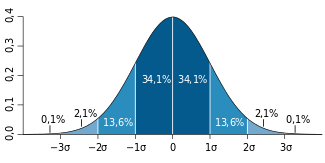
\includegraphics[scale=1]{pics/3sigm.png}}
\caption{правило трех сигм \cite{3}}
\end{figure}

Поскольку у нормального распределения $\sqrt {n} N(0,1)$ среднеквадратичное отклонение $\sigma = \sqrt{n}$, по правилу трех сигм можно сказать, что у центрального пути длины $n-2f(n)$ вероятность остановиться в промежутке $[-3\sqrt{n-2f(n)}; 3\sqrt{n-2f(n)}]$ около 0.9973, а поскольку $f(n)=o(n)$, вероятность того, что изменение координаты окажется вне промежутка $[-2.5\sqrt{n}; 2.5\sqrt{n}]$, хотя бы 0.0026.

Для того, чтобы получить отрезок длины $n-f(n)$ с нулевой суммой, нужно взять какой-то суффикс префикса длины $f(n)$ и какой-то префикс суффикса длины $f(n)$. Покажем, что с достаточной вероятностью мы не сможем приблизиться к нулю за $f(n)$ шагов.

Скажем, что наше блуждание сейчас будет обычным случайным, с двумя переходами $+1$ и $-1$. Этот переход является корректным, так как если в обычном случайном блуждании утверждение выполнено, то оно верно и для нашего случая. И действительно, можно продлить все испытания, в которых был переход по 0 до ровно $k$ (общее число испытаний) ненулевых переходов и прийти к случайному блужданию, при чем максимум модуля отклонения на префиксе мог только увеличиться.

Поскольку $2f(n)=o(n)$, докажем более сильное условие. За $n$ шагов с вероятностью $C>0$, не зависящей от $n$, случайное блуждание не попадет в область с координатой меньше $-\sqrt{n}$. 

Переформулируем эту задачу как задачу о разорении: игрок имеет $\sqrt{n}$ денег и играет $n$ раундов против бесконечно богатого казино, и нужно найти вероятность разорения игрока. В \cite{7} и в \cite{8} можно найти следующую формулу: вероятность проигрыша игрока со стартовым капиталом $a$ за $n$ раундов равна $y_{a,n}=1-{{2} \over {\sqrt{\pi}}} \int_0^t e^{-u^2} du + \Delta$, где $\Delta$~--- малый остаточный член, а $t={{a} \over {\sqrt{2(n+{{2}\over 3})}}}$.

В нашем случае, $a=\sqrt n$, $t \approx {1 \over \sqrt 2}$, и вероятность проигрыша в пределе равна $1 - {2 \over \sqrt \pi} \int_0^{1 \over \sqrt 2} e^{-u^2} du \approx 0.395$.

Таким образом, с вероятностью хотя бы 0.0026 центральный подпуть будет иметь отклонение от нуля хотя бы в $2.5\sqrt n$, и с вероятностью хотя бы $0.605^2$ и префикс, и суффикс, который мы допишем к этой строке, будут иметь отклонение не больше, чем на $\sqrt n$, то есть, с вероятностью $P \ge 0.026 \cdot 0.605^2$ у двух случайных строк наибольшая Абелева подстрока будет меньше, чем $n-f(n)$.

\end{proof}

Вернемся к доказательству теоремы. Будем доказывать ее от противного~--- пусть есть $f(n)=o(n)$ такое, что $LCAF_{avg} \ge n - f(n)$. 

Оценим $LCAF_{avg}$. По лемме, с вероятностью $0.026 \cdot 0.605^2 = 0.0095$ $LCAF$ будет не больше, чем $g(n)=\sqrt{nf(n)}$. Тогда

$LCAF_{avg} \le 0.0095 \cdot (n-g(n)) + (1-0.0095)\cdot n = n-0.0095\cdot g(n) < n - f(n)$, т.к. $f=o(g)$. Противоречие.

\end{proof}

Кроме того, докажем грубую оценку снизу:
\begin{theorem}
Для двух случайных бинарных строк длины $n$: $LCAF_{avg} \ge 0.05n$.
\end{theorem}
\begin{proof}
Снова приблизим наше случайное блуждание нормальным распределением и воспользуемся правилом трех сигм.

С вероятностью $2 \cdot 0.34$ за первые $n/2$ шагов мы остановимся в зоне $[-\sqrt{n \over 2}; \sqrt{n \over 2}]$. После этого, с вероятностью хотя бы $0.136+0.021+0.001 \ge 0.15$ (вероятность пройти в нужную сторону больше, чем $\sqrt{n \over 2}$ шагов, см. рисунок 1) мы за следующие $n/2$ шагов пройдем в другую сторону хотя бы $\sqrt{n \over 2}$ шагов, обязательно перейдя через точку старта. Таким образом, с вероятностью хотя бы $2 \cdot 0.34 \cdot 0.15$ НОАП будет хотя бы $n/2$, или $LCAF_{avg} \ge 0.05$. %TODO может стоит \sigma -> \sqrt

\end{proof}

Итого, получаем, что матожидание НОАП у двух случайных бинарных строк сверху и снизу ограничено линейными функциями, но более точная оценка ее поведения остается нерешенной задачей.

\subsubsection{Сведение к 3SUM+}

Можно получить асимптотически хорошее решение, использовав алгоритм решения $3SUM^+$, описанный в \cite{2}. 

В упомянутой статье было предложено \textbf{Corollary 3.6}, позволяющее решать задачу \textit{histogram indexing} для случая бинарной строки за предподсчет $\mathcal{O}(n^{1.86})$, и отвечать после этого на запрос за $\mathcal{O}(1)$. В процессе предподсчета оказываются посчитаны значения минимального и максимального количества вхождений $c_0$ в строку длины $l$ для каждой длины $l$. Используя эти массивы можно найти НОАП, перебрав длину $l$ общей подстроки, проверив, пересекаются ли множества подстрок длины $l$ с фиксированным количеством вхождений у обеих строк, и выбрав наибольшее подходящее $l$.

Используя это сведение, получаем решение задачи поиска НОАП для бинарного алфавита за $\mathcal{O}(n^{1.86})$, лучшее на данный момент.
%\end{table}